\section{Simulation}
\markright{Simulation}

A DC sweep simulation was included to compare the ideal circuit response with the
laboratory observation. The simulated circuit used a 1N4007 silicon diode in
series with a $10\,\text{k}\Omega$ resistor and a variable DC source. The source
voltage was swept from $0.1$ to $1.5\,\text{V}$ for forward bias and from $2$ to
$11.5\,\text{V}$ for reverse bias. The expected current was obtained from the
series relation
\[
  I_D = \frac{V_S - V_D}{R}
\]
with $R = 10\,\text{k}\Omega$, along with the nonlinear diode behavior.

\begin{figure}
  \begin{subfigure}[b]{\textwidth}
    \centering
    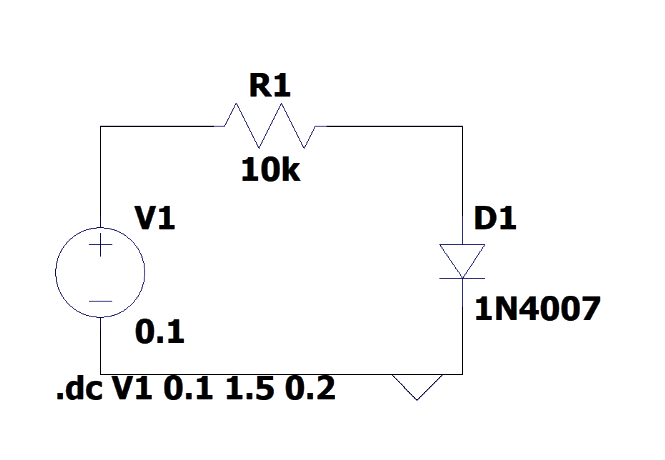
\includegraphics[width=\textwidth, height=5cm, keepaspectratio]{lab-02/schematics/fb-diagram.png}
    \caption{Schematic}
  \end{subfigure}
  \hfil
  \begin{subfigure}[b]{\textwidth}
    \centering
    
\includegraphics[width=\textwidth, height=5cm, keepaspectratio]{lab-02/schematics/fb-graph.png}
    \caption{Graph}
  \end{subfigure}
  \caption{Showing the forward-bias simulation.}
  \label{lab2_sim_forward}
\end{figure}


\begin{figure}
  \begin{subfigure}[b]{0.45\textwidth}
    \centering
    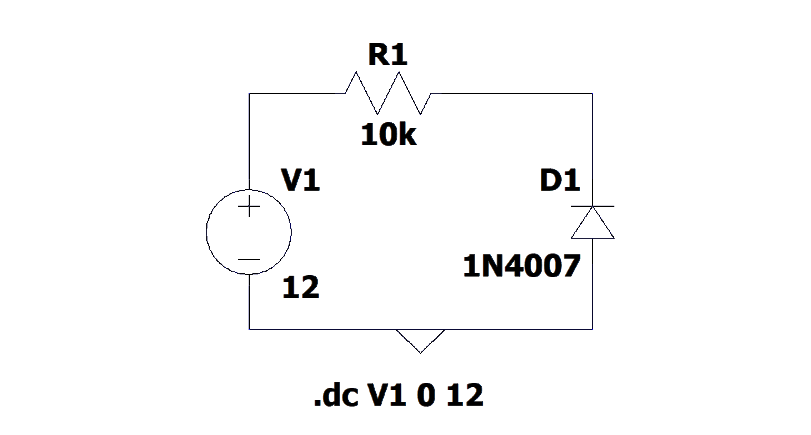
\includegraphics[width=\textwidth, height=5cm, keepaspectratio]{lab-02/schematics/rb-diagram.png}
    \caption{Schematic}
  \end{subfigure}
  \hfil
  \begin{subfigure}[b]{0.5\textwidth}
    \centering
    
\includegraphics[width=\textwidth, height=5cm, keepaspectratio]{lab-02/schematics/rb-graph.png}
    \caption{Graph}
  \end{subfigure}
  \caption{Showing the reverse-bias simulation.}
  \label{lab2_sim_reverse}
\end{figure}
